%!TEX TS-program = xelatex
%!TEX encoding = UTF-8 Unicode

%% bare_conf.tex
%% V1.4a
%% 2014/09/17
%% by Michael Shell
%% See:
%% http://www.michaelshell.org/
%% for current contact information.
%%
%% This is a skeleton file demonstrating the use of IEEEtran.cls
%% (requires IEEEtran.cls version 1.8a or later) with an IEEE
%% conference paper.
%%
%% Support sites:
%% http://www.michaelshell.org/tex/ieeetran/
%% http://www.ctan.org/tex-archive/macros/latex/contrib/IEEEtran/
%% and
%% http://www.ieee.org/

%%*************************************************************************
%% Legal Notice:
%% This code is offered as-is without any warranty either expressed or
%% implied; without even the implied warranty of MERCHANTABILITY or
%% FITNESS FOR A PARTICULAR PURPOSE! 
%% User assumes all risk.
%% In no event shall IEEE or any contributor to this code be liable for
%% any damages or losses, including, but not limited to, incidental,
%% consequential, or any other damages, resulting from the use or misuse
%% of any information contained here.
%%
%% All comments are the opinions of their respective authors and are not
%% necessarily endorsed by the IEEE.
%%
%% This work is distributed under the LaTeX Project Public License (LPPL)
%% ( http://www.latex-project.org/ ) version 1.3, and may be freely used,
%% distributed and modified. A copy of the LPPL, version 1.3, is included
%% in the base LaTeX documentation of all distributions of LaTeX released
%% 2003/12/01 or later.
%% Retain all contribution notices and credits.
%% ** Modified files should be clearly indicated as such, including  **
%% ** renaming them and changing author support contact information. **
%%
%% File list of work: IEEEtran.cls, IEEEtran_HOWTO.pdf, bare_adv.tex,
%%                    bare_conf.tex, bare_jrnl.tex, bare_conf_compsoc.tex,
%%                    bare_jrnl_compsoc.tex, bare_jrnl_transmag.tex
%%*************************************************************************


% *** Authors should verify (and, if needed, correct) their LaTeX system  ***
% *** with the testflow diagnostic prior to trusting their LaTeX platform ***
% *** with production work. IEEE's font choices and paper sizes can       ***
% *** trigger bugs that do not appear when using other class files.       ***                          ***
% The testflow support page is at:
% http://www.michaelshell.org/tex/testflow/



\documentclass[conference]{IEEEtran}

% Some Computer Society conferences also require the compsoc mode option,
% but others use the standard conference format.
%
% If IEEEtran.cls has not been installed into the LaTeX system files,
% manually specify the path to it like:
% \documentclass[conference]{../sty/IEEEtran}





% Some very useful LaTeX packages include:
% (uncomment the ones you want to load)


% *** MISC UTILITY PACKAGES ***
%
%\usepackage{ifpdf}
% Heiko Oberdiek's ifpdf.sty is very useful if you need conditional
% compilation based on whether the output is pdf or dvi.
% usage:
% \ifpdf
%   % pdf code
% \else
%   % dvi code
% \fi
% The latest version of ifpdf.sty can be obtained from:
% http://www.ctan.org/tex-archive/macros/latex/contrib/oberdiek/
% Also, note that IEEEtran.cls V1.7 and later provides a builtin
% \ifCLASSINFOpdf conditional that works the same way.
% When switching from latex to pdflatex and vice-versa, the compiler may
% have to be run twice to clear warning/error messages.






% *** CITATION PACKAGES ***
%
%\usepackage{cite}
% cite.sty was written by Donald Arseneau
% V1.6 and later of IEEEtran pre-defines the format of the cite.sty package
% \cite{} output to follow that of IEEE. Loading the cite package will
% result in citation numbers being automatically sorted and properly
% "compressed/ranged". e.g., [1], [9], [2], [7], [5], [6] without using
% cite.sty will become [1], [2], [5]--[7], [9] using cite.sty. cite.sty's
% \cite will automatically add leading space, if needed. Use cite.sty's
% noadjust option (cite.sty V3.8 and later) if you want to turn this off
% such as if a citation ever needs to be enclosed in parenthesis.
% cite.sty is already installed on most LaTeX systems. Be sure and use
% version 5.0 (2009-03-20) and later if using hyperref.sty.
% The latest version can be obtained at:
% http://www.ctan.org/tex-archive/macros/latex/contrib/cite/
% The documentation is contained in the cite.sty file itself.



\usepackage{algorithm}
\usepackage{algpseudocode}
\usepackage{amsmath}
\usepackage{graphicx}
% *** GRAPHICS RELATED PACKAGES ***
%
%\ifCLASSINFOpdf
  % \usepackage[pdftex]{graphicx}
  % declare the path(s) where your graphic files are
  % \graphicspath{{../pdf/}{../jpeg/}}
  % and their extensions so you won't have to specify these with
  % every instance of \includegraphics
  % \DeclareGraphicsExtensions{.pdf,.jpg,.png}
%\else
  % or other class option (dvipsone, dvipdf, if not using dvips). graphicx
  % will default to the driver specified in the system graphics.cfg if no
  % driver is specified.
  % \usepackage[dvips]{graphicx}
  % declare the path(s) where your graphic files are
  % \graphicspath{{../eps/}}
  % and their extensions so you won't have to specify these with
  % every instance of \includegraphics
  % \DeclareGraphicsExtensions{.eps}
%\fi
% graphicx was written by David Carlisle and Sebastian Rahtz. It is
% required if you want graphics, photos, etc. graphicx.sty is already
% installed on most LaTeX systems. The latest version and documentation
% can be obtained at: 
% http://www.ctan.org/tex-archive/macros/latex/required/graphics/
% Another good source of documentation is "Using Imported Graphics in
% LaTeX2e" by Keith Reckdahl which can be found at:
% http://www.ctan.org/tex-archive/info/epslatex/
%
% latex, and pdflatex in dvi mode, support graphics in encapsulated
% postscript (.eps) format. pdflatex in pdf mode supports graphics
% in .pdf, .jpeg, .png and .mps (metapost) formats. Users should ensure
% that all non-photo figures use a vector format (.eps, .pdf, .mps) and
% not a bitmapped formats (.jpeg, .png). IEEE frowns on bitmapped formats
% which can result in "jaggedy"/blurry rendering of lines and letters as
% well as large increases in file sizes.
%
% You can find documentation about the pdfTeX application at:
% http://www.tug.org/applications/pdftex




\newcommand{\pluseq}{\mathrel{+}=}
\newcommand{\asteq}{\mathrel{*}=}

% *** MATH PACKAGES ***
%
%\usepackage[cmex10]{amsmath}
% A popular package from the American Mathematical Society that provides
% many useful and powerful commands for dealing with mathematics. If using
% it, be sure to load this package with the cmex10 option to ensure that
% only type 1 fonts will utilized at all point sizes. Without this option,
% it is possible that some math symbols, particularly those within
% footnotes, will be rendered in bitmap form which will result in a
% document that can not be IEEE Xplore compliant!
%
% Also, note that the amsmath package sets \interdisplaylinepenalty to 10000
% thus preventing page breaks from occurring within multiline equations. Use:
%\interdisplaylinepenalty=2500
% after loading amsmath to restore such page breaks as IEEEtran.cls normally
% does. amsmath.sty is already installed on most LaTeX systems. The latest
% version and documentation can be obtained at:
% http://www.ctan.org/tex-archive/macros/latex/required/amslatex/math/




% *** SPECIALIZED LIST PACKAGES ***
%
%\usepackage{algorithmic}
% algorithmic.sty was written by Peter Williams and Rogerio Brito.
% This package provides an algorithmic environment fo describing algorithms.
% You can use the algorithmic environment in-text or within a figure
% environment to provide for a floating algorithm. Do NOT use the algorithm
% floating environment provided by algorithm.sty (by the same authors) or
% algorithm2e.sty (by Christophe Fiorio) as IEEE does not use dedicated
% algorithm float types and packages that provide these will not provide
% correct IEEE style captions. The latest version and documentation of
% algorithmic.sty can be obtained at:
% http://www.ctan.org/tex-archive/macros/latex/contrib/algorithms/
% There is also a support site at:
% http://algorithms.berlios.de/index.html
% Also of interest may be the (relatively newer and more customizable)
% algorithmicx.sty package by Szasz Janos:
% http://www.ctan.org/tex-archive/macros/latex/contrib/algorithmicx/




% *** ALIGNMENT PACKAGES ***
%
%\usepackage{array}
% Frank Mittelbach's and David Carlisle's array.sty patches and improves
% the standard LaTeX2e array and tabular environments to provide better
% appearance and additional user controls. As the default LaTeX2e table
% generation code is lacking to the point of almost being broken with
% respect to the quality of the end results, all users are strongly
% advised to use an enhanced (at the very least that provided by array.sty)
% set of table tools. array.sty is already installed on most systems. The
% latest version and documentation can be obtained at:
% http://www.ctan.org/tex-archive/macros/latex/required/tools/


% IEEEtran contains the IEEEeqnarray family of commands that can be used to
% generate multiline equations as well as matrices, tables, etc., of high
% quality.




% *** SUBFIGURE PACKAGES ***
%\ifCLASSOPTIONcompsoc
%  \usepackage[caption=false,font=normalsize,labelfont=sf,textfont=sf]{subfig}
%\else
%  \usepackage[caption=false,font=footnotesize]{subfig}
%\fi
% subfig.sty, written by Steven Douglas Cochran, is the modern replacement
% for subfigure.sty, the latter of which is no longer maintained and is
% incompatible with some LaTeX packages including fixltx2e. However,
% subfig.sty requires and automatically loads Axel Sommerfeldt's caption.sty
% which will override IEEEtran.cls' handling of captions and this will result
% in non-IEEE style figure/table captions. To prevent this problem, be sure
% and invoke subfig.sty's "caption=false" package option (available since
% subfig.sty version 1.3, 2005/06/28) as this is will preserve IEEEtran.cls
% handling of captions.
% Note that the Computer Society format requires a larger sans serif font
% than the serif footnote size font used in traditional IEEE formatting
% and thus the need to invoke different subfig.sty package options depending
% on whether compsoc mode has been enabled.
%
% The latest version and documentation of subfig.sty can be obtained at:
% http://www.ctan.org/tex-archive/macros/latex/contrib/subfig/




% *** FLOAT PACKAGES ***
%
%\usepackage{fixltx2e}
% fixltx2e, the successor to the earlier fix2col.sty, was written by
% Frank Mittelbach and David Carlisle. This package corrects a few problems
% in the LaTeX2e kernel, the most notable of which is that in current
% LaTeX2e releases, the ordering of single and double column floats is not
% guaranteed to be preserved. Thus, an unpatched LaTeX2e can allow a
% single column figure to be placed prior to an earlier double column
% figure. The latest version and documentation can be found at:
% http://www.ctan.org/tex-archive/macros/latex/base/


%\usepackage{stfloats}
% stfloats.sty was written by Sigitas Tolusis. This package gives LaTeX2e
% the ability to do double column floats at the bottom of the page as well
% as the top. (e.g., "\begin{figure*}[!b]" is not normally possible in
% LaTeX2e). It also provides a command:
%\fnbelowfloat
% to enable the placement of footnotes below bottom floats (the standard
% LaTeX2e kernel puts them above bottom floats). This is an invasive package
% which rewrites many portions of the LaTeX2e float routines. It may not work
% with other packages that modify the LaTeX2e float routines. The latest
% version and documentation can be obtained at:
% http://www.ctan.org/tex-archive/macros/latex/contrib/sttools/
% Do not use the stfloats baselinefloat ability as IEEE does not allow
% \baselineskip to stretch. Authors submitting work to the IEEE should note
% that IEEE rarely uses double column equations and that authors should try
% to avoid such use. Do not be tempted to use the cuted.sty or midfloat.sty
% packages (also by Sigitas Tolusis) as IEEE does not format its papers in
% such ways.
% Do not attempt to use stfloats with fixltx2e as they are incompatible.
% Instead, use Morten Hogholm'a dblfloatfix which combines the features
% of both fixltx2e and stfloats:
%
% \usepackage{dblfloatfix}
% The latest version can be found at:
% http://www.ctan.org/tex-archive/macros/latex/contrib/dblfloatfix/




% *** PDF, URL AND HYPERLINK PACKAGES ***
%
\usepackage{url}
% url.sty was written by Donald Arseneau. It provides better support for
% handling and breaking URLs. url.sty is already installed on most LaTeX
% systems. The latest version and documentation can be obtained at:
% http://www.ctan.org/tex-archive/macros/latex/contrib/url/
% Basically, \url{my_url_here}.




% *** Do not adjust lengths that control margins, column widths, etc. ***
% *** Do not use packages that alter fonts (such as pslatex).         ***
% There should be no need to do such things with IEEEtran.cls V1.6 and later.
% (Unless specifically asked to do so by the journal or conference you plan
% to submit to, of course. )


% correct bad hyphenation here
\hyphenation{op-tical net-works semi-conduc-tor}

\begin{document}
%
% paper title
% Titles are generally capitalized except for words such as a, an, and, as,
% at, but, by, for, in, nor, of, on, or, the, to and up, which are usually
% not capitalized unless they are the first or last word of the title.
% Linebreaks \\ can be used within to get better formatting as desired.
% Do not put math or special symbols in the title.
\title{Topic-Aware Sentiment Prediction for Chinese ConceptNet}


% author names and affiliations
% use a multiple column layout for up to three different
% affiliations
\author{\IEEEauthorblockN{Po-Hao Chou}
\IEEEauthorblockA{Department of CSIE,\\National Taiwan University\\
Taipei, Taiwan\\
Email: r02922017@ntu.edu.tw}
\and
\IEEEauthorblockN{Chi-Chia Huang}
\IEEEauthorblockA{Department of CSIE,\\National Taiwan University\\
Taipei, Taiwan\\
Email: }
\and
\IEEEauthorblockN{James Kirk\\ and Montgomery Scott}
\IEEEauthorblockA{Starfleet Academy\\
San Francisco, California 96678--2391\\
Telephone: (800) 555--1212\\
Fax: (888) 555--1212}}

% conference papers do not typically use \thanks and this command
% is locked out in conference mode. If really needed, such as for
% the acknowledgment of grants, issue a \IEEEoverridecommandlockouts
% after \documentclass

% for over three affiliations, or if they all won't fit within the width
% of the page, use this alternative format:
% 
%\author{\IEEEauthorblockN{Michael Shell\IEEEauthorrefmark{1},
%Homer Simpson\IEEEauthorrefmark{2},
%James Kirk\IEEEauthorrefmark{3}, 
%Montgomery Scott\IEEEauthorrefmark{3} and
%Eldon Tyrell\IEEEauthorrefmark{4}}
%\IEEEauthorblockA{\IEEEauthorrefmark{1}School of Electrical and Computer Engineering\\
%Georgia Institute of Technology,
%Atlanta, Georgia 30332--0250\\ Email: see http://www.michaelshell.org/contact.html}
%\IEEEauthorblockA{\IEEEauthorrefmark{2}Twentieth Century Fox, Springfield, USA\\
%Email: homer@thesimpsons.com}
%\IEEEauthorblockA{\IEEEauthorrefmark{3}Starfleet Academy, San Francisco, California 96678-2391\\
%Telephone: (800) 555--1212, Fax: (888) 555--1212}
%\IEEEauthorblockA{\IEEEauthorrefmark{4}Tyrell Inc., 123 Replicant Street, Los Angeles, California 90210--4321}}




% use for special paper notices
%\IEEEspecialpapernotice{(Invited Paper)}




% make the title area
\maketitle

% As a general rule, do not put math, special symbols or citations
% in the abstract
\begin{abstract}
Sentiment analysis aims to identify the attitudes or emotions behind texts. For many sentiment analysis approaches, sentiment information of terms or phrases plays an important role. However, in Chinese sentiment analysis, the coverage of such information is still limited. To increase the coverage, some methods has been developed to predict sentiments for nodes in Chinese ConceptNet due to its large size and high semantic level nodes. In ConceptNet, the notion of a node is extended from purely lexical terms to include higher-order compound concepts, e.g., 'eat lunch', 'satisfy hunger', so these nodes are called concepts. 

Current approaches aim to assign one sentiment to each concept, but in fact a concept may have different sentiments on different contexts, such as 'scream' and 'sudden' in Chinese. In this paper, our first goal is to extract the hidden contextual information in Chinese ConceptNet and use it to estimate sentiments in different situations for each concept. To achieve this goal, we propose a topic-aware sentiment propagation approach. We apply Latent Dirichlet Allocation to divide Chinese ConceptNet into different topic layers and use sentiment propagation on each topic layer to predict topic-aware sentiments for Chinese concepts. Our another goal is to use the generated topic-aware sentiments of concepts to improve the polarity classification for texts. We combine other co-occurring concepts to identify topics and select sentiments for concepts in texts. Then, experiments conducted on dialogue dataset and microblog posts show the improvement of topic-aware prediction for concepts and texts. 
\end{abstract}

% no keywords




% For peer review papers, you can put extra information on the cover
% page as needed:
% \ifCLASSOPTIONpeerreview
% \begin{center} \bfseries EDICS Category: 3-BBND \end{center}
% \fi
%
% For peerreview papers, this IEEEtran command inserts a page break and
% creates the second title. It will be ignored for other modes.
\IEEEpeerreviewmaketitle



\section{Introduction}
With the rise of social media services, more and more people share their opinions, feelings, experiences on the web. The roles of users shift from information consumers to information producers. To understand the attitudes and emotions behind these texts, sentiment analysis has become a popular research topic in recent years. 

Sentiment dictionaries tell machine how a writer or speaker may feel when using some term or phrase. They are important elements for several sentiment analysis approaches~\cite{Taboada:lexiconBased11, Rao:WWW14, Wen:AAAI14, Lee:IJCNLP2011}, but in Chinese, they are relatively scarce or non-public. As the result, it is helpful to collect the sentiment information in Chinese. However, there are two problems in collecting sentiment information. First, its coverage and quality highly affect the performance of sentiment analysis for texts, but collecting the information with high coverage, quality but low cost is challenging. The second problem is that the sentiments of several terms and phrases are context-dependent. How to define context, collect the sentiments on different contexts efficiently and decide which context and sentiment should be used to predict sentiments of texts are challenges.

For the first problem, several approaches~\cite{Strapparava:IREC04, Esuli:LREC06, Liu:IUI03, Cambria:AAAI10, Wu:TAAI11, Tsai:IEEE13, Wu:relSelect14} have used the external knowledge such as WordNet~\cite{Miller:WordNet95} and ConceptNet~\cite{Havasi:RANLP07,Speer:LREC12} to build sentiment dictionaries automatically. The relationship information in WordNet and ConceptNet is used to propagate sentiments from some seeds, which had been compiled manually. 

ConceptNet is a semantic network which represents knowledge into more computable representations. The nodes in ConceptNet are called {\it concepts} because the coverage of nodes contains not only lexical terms but also higher-order compound concepts, e.g., 'accomplish goal', 'leave behind'. A directed edge connecting two nodes is called {\it relation}, and is associated with one of the predefined types of labels to represent the semantic relationships between two {\it concepts} in real world, e.g., 'CapableOf', 'Causes'. The former {\it concept}, latter {\it concept} and their {\it relation} form an {\it assertion}, such as ``oven UsedFor cook", ``eat HasSubevent swallow". Because ConceptNet has large amount of {\it concepts} (In Chinese part~\cite{Kuo:HCOMP09,Kuo:FSS10}, there are at least 220000 {\it concepts}, still growing...), and its {\it concepts} have higher semantic meaning than traditional lexical terms, it is a good foundation to build a larger sentiment dictionary. In this paper, we collect sentiments based on {\it concepts} and the structure in Chinese ConceptNet.

However, previous propagation approaches in ConceptNet didn't deal with the issue that a {\it concept}'s neighbors may come from different scenarios. Take Figure~\ref{fig:noWork2} for example, previous approaches aggregate the sentiments from neighbors disregarding their different scenarios, and assign the aggregated sentiment to 'do not have to work'. 'do dot have to work' will propagate this sentiment to all its neighbors in the next iteration, which makes sentiments be propagated between different scenarios.

\begin{figure}[!t]
\centering
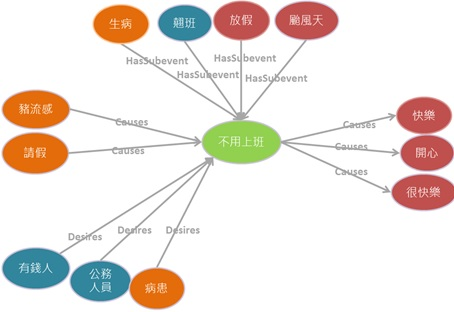
\includegraphics[width=2.5in]{fig/noWork2.jpg}
\caption{Neighbors of 'do not have to work' come from different scenarios.}
\label{fig:noWork2}
\end{figure}

The second problem is that each {\it concept} should be assigned different sentiments in different scenarios. For example, 'scream' is more possible to be negative when 'pervert' or 'cockroach' appears, but is more likely to be positive when 'idol' or 'win' appears. Previous approaches ~\cite{Xu:PACLIC10, Xu:COLING10, Rao:WWW14} use domain-specific corpus to modify sentiment value according to the corpus. However, hidden contextual information in Chinese ConceptNet is also abundant, like Figure~\ref{fig:noWork2}. If we could know which scenario an assertion belongs to, a {\it concept}'s sentiment in a scenario can be determined from its assertions which belongs to the scenario. 

To deal with the two problems, this paper develops a topic-aware propagation method for Chinese ConceptNet. We extract hidden contextual information by applying Latent Dirichlet Allocation~\cite{Blei:LDA03} to Chinese ConceptNet. Then we use the information to improve original sentiment propagation and predict topic-aware sentiment values for {\it concepts}. Then we present how to apply these topic-aware sentiment values of {\it concepts} to polarity classification for texts. Finally, experiments are conducted on dialogue dataset and microblog posts benchmark.


\section{Related Work}
\subsection{Sentiment Prediction for ConceptNet}
Random walk is commonly used to spread values on a graph~\cite{Wu:relSelect14,Hassan:ACL10,Xu:COLING10,Cambria:AAAI10}. It spreads values through synonym and antonym edges. The equation of random walk with restart is as follows:
\begin{equation}
\label{eq:rndWalk}
\boldsymbol{s}_{t+1} = (1-\alpha)\boldsymbol{W}\boldsymbol{s}_t + \alpha\boldsymbol{s}_0
\end{equation}
where $\boldsymbol{s}_t$ is the values of each node when the $t$-th iteration. $\boldsymbol{W}$ is a similarity matrix, which can be acquired from sources like Ontology, ConceptNet, corpus, etc. Similarity matrix of a standard random walk is an out-link normalized matrix. $\alpha$ is the restarting weight. Random walk is an iterative process, and after $n$ iteration, each node spreads its value to the neighbors that are $n$ links distant from it.

In previous research~\cite{Tsai:IEEE13, Wu:relSelect14}, random walk is applied to propagate values on ConceptNet. They found that in ConceptNet, performing in-link normalized on similarity matrix is better than performing out-link normalized because out-link normalization will underestimate the influence of concepts with more neighbors. In in-link normalization, each concept's new sentiment value in the ($t+1$)-th iteration is the average of all its neighbors in the $t$-th iteration.

\subsection{Latent Dirichlet Allocation}
Latent Dirichlet Allocation (LDA)~\cite{Blei:LDA03} is a generative probabilistic model of a corpus, in which documents are represented as random mixtures over latent topics, and each topic is characterized by a distribution over words. The intuition behind LDA is that each document exhibits multiple topics. It exploits word co-occurrence information to capture latent topics in the corpus.

In LDA, each document $d$ is represented by bag of words (so the order of words in a document is not considered), and each document is assumed to be generated by the following (given parameters of Dirichlet distribution $\boldsymbol{\alpha}$ and per-topic word distribution $\boldsymbol{\beta}$):
\begin{enumerate}[]
	\item Choose probability coefficients over topics $\boldsymbol{\theta}_d {\sim} Dir(\boldsymbol{\alpha})$
	\item For each of the $N$ word positions $x_{d,n}$:
	\begin{enumerate}
		\item Choose a topic assignment $z_{d,n} {\sim} Multinomial(\boldsymbol{\theta})$
		\item Choose a word $w_{d,n}$ conditioned on the chosen topic $z_{d,n}$ and the per-topic word distribution $\boldsymbol{\beta}_{z_{d,n}}$
	\end{enumerate}
\end{enumerate}

From the generative process, the graphical model representation of basic LDA is shown in Figure~\ref{fig:LDA_model}. Observing word co-occurrence in each document, LDA infers topic probability coefficients $\boldsymbol{\theta}_d$ for each document and topic assignment $z_{d,n}$ for each word of each document to maximize the likelihood of this corpus. However, the posterior distribution is intractable for exact inference of each $\boldsymbol{theta}_d$ and $z_{d,n}$. Blei {\it et al.} use variational EM to infer these latent variables and find parameters $\boldsymbol{\alpha}$ and $\boldsymbol{\beta}$ to maximize the log likelihood of given corpus.

\begin{figure}[!t]
\centering
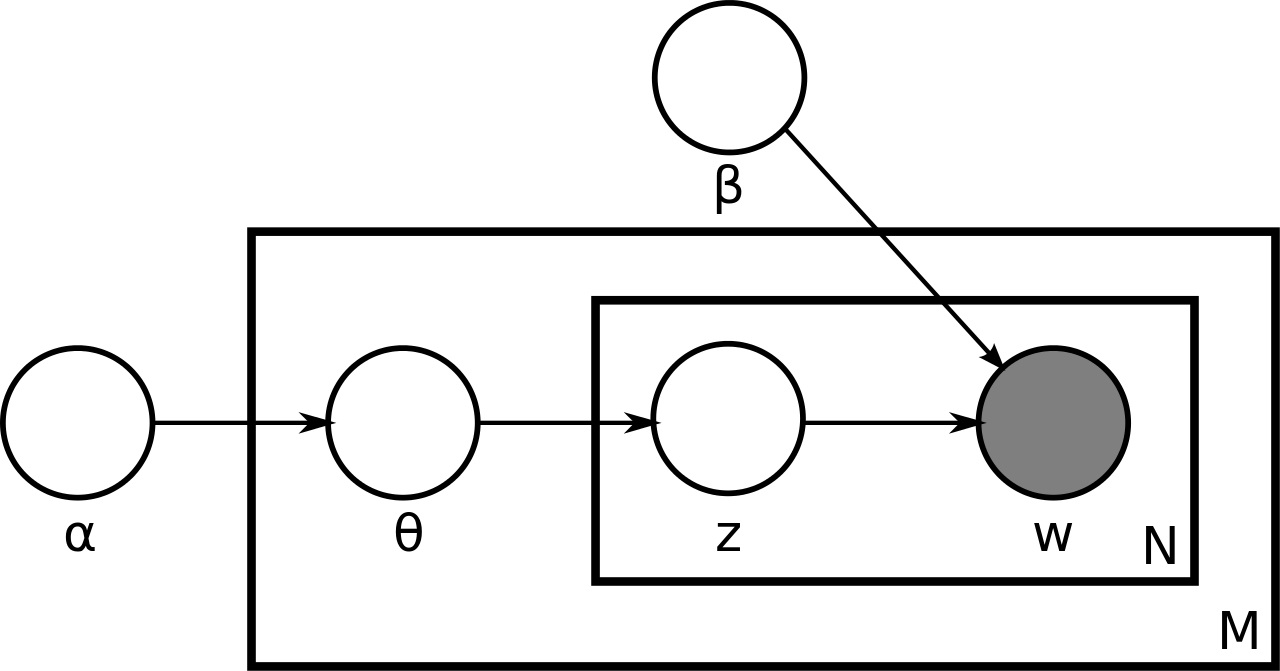
\includegraphics[width=2.5in]{fig/LDA_model.jpg}
\caption{Graphical model representation of LDA.}
\label{fig:LDA_model}
\end{figure}

Because the words coverage for each document is sparse, they smooth multinomial parameters $\boldsymbol{\beta}$ by generating $\boldsymbol{\beta}_k \sim Dir(\boldsymbol{\eta})$ for each topic, shown in Figure~\ref{fig:LDA_model2}. They infer $\boldsymbol{\beta}_k$ by modify the variational model, like inferring $\boldsymbol{\theta}_d$.

\begin{figure}[!t]
\centering
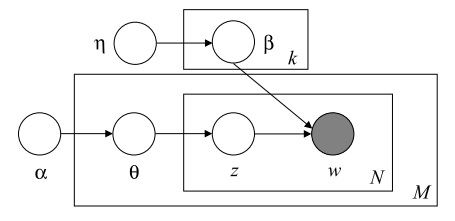
\includegraphics[width=2.5in]{fig/LDA_model2.jpg}
\caption{Graphical model representation of smoothed LDA.}
\label{fig:LDA_model2}
\end{figure}

As the result, LDA infers $\boldsymbol{\theta}_d$ for each document, $z_{d,n}$ for each word of document and $\boldsymbol{\beta}_k$ for each topic. Besides, it estimates $\boldsymbol{\alpha}$ and $\boldsymbol{\eta}$ as the model of this corpus.


%==========================================
\section{Topic-Aware Sentiment Value Prediction for Chinese ConceptNet}
In topic models such as LDA, each abstract ``topic" is characterized by a distribution over words. Such topics are one kind of representation of contexts or scenarios. In this section, we aim to define the topics in Chinese ConceptNet and predict a sentiment value $\in [-1,1]$ on each topic for each concept. Figure~\ref{fig:system1} shows the architecture of our system.

\begin{figure}[!t]
\centering
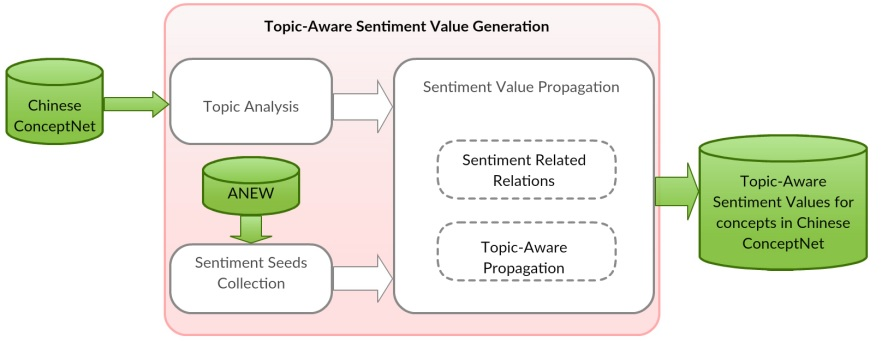
\includegraphics[width=0.5\textwidth]{fig/system1.jpg}
\caption{System Architecture.}
\label{fig:system1}
\end{figure}

\subsection{Topic Analysis on ConceptNet}
We choose LDA to estimate topics for two reasons: The first one is that LDA allows each document to exhibit multiple topics to different degrees. The second one is that there are corpus parameters after LDA estimation, and we can use these corpus parameters to infer a new document by running the E-step in LDA. 

Similar to the assumption of generating a corpus in LDA, we assume that there is a topic distribution for each concept and its assertions are sampled from this distribution. We aim to find which topic each assertion comes from for each concept. Therefore, we try to apply LDA to find such latent information. 

First, each concept forms a document using its neighbors such that these neighbors have one co-occurrence observation when LDA estimates. See Figure~\ref{fig:noWorkDoc} for illustration, the concept 'do not have to work' generates a document using neighbors as words, with a value indicating how many times the neighbor occurs in assertions.

\begin{figure}[!t]
\centering
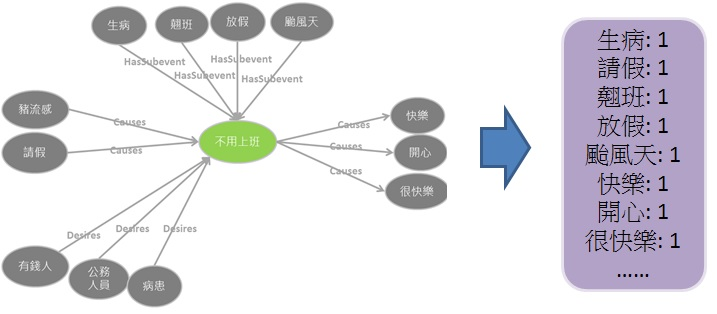
\includegraphics[width=0.5\textwidth]{fig/noWorkDoc.jpg}
\caption{The document generated by 'do not have to work'.}
\label{fig:noWorkDoc}
\end{figure}

Then we apply LDA to find $\boldsymbol{\theta}_m$ for each document d$_m$ and $z_{m,n}$ for each word $w_{m,n}$ in d$_m$ based on this collection of $M$ documents. Words in each document stand for neighbors of concept, so each resulted $z_{m,n}$ indicates which topicID the neighbor $w_{m,n}$ comes from for concept $c_m$.

As the result, we can design a topic assignment matrix, $\boldsymbol{T}$ where each entry $t_{i,j}$ is $z_{i,j}$ if $j$ is one of $i$'s neighbors, otherwise $unknown$. That is, we can check $t_{i,j}$ for which topicID $i$'s neighbor $j$ belongs to. 

Here we present the result of applying LDA with 10 topics to Chinese ConceptNet. Figure~\ref{fig:wordTop20} shows the per-topic word distribution, $\boldsymbol{\beta}_k$. Each column shows the top 20 words of a topic.

\begin{figure}[!t]
\centering
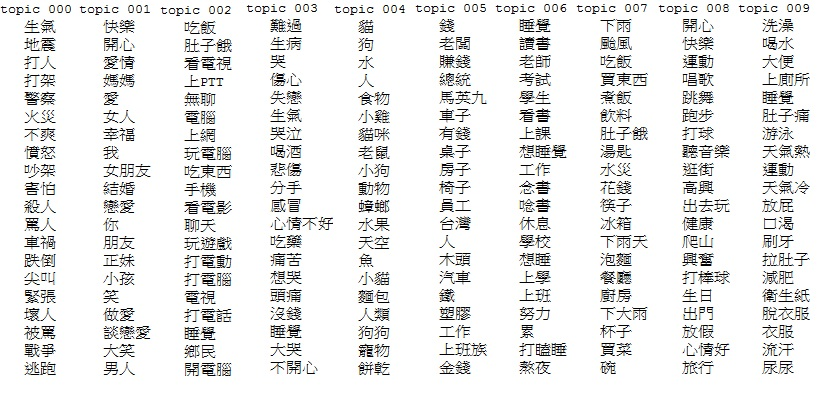
\includegraphics[width=0.5\textwidth]{fig/wordTop20.jpg}
\caption{The top 20 words of each topic.}
\label{fig:wordTop20}
\end{figure}

\subsection{Collecting Sentiment Seeds}
Sentiment seeds here are concepts whose sentiments are known. Common ways to collect sentiment seeds are compiling manually or using other existing sentiment dictionaries. Although concepts we consider here are in Chinese, we use words in Affective Norms for English Words (ANEW)~\cite{Bradley:ANEW99} as our seeds. One reason is its good quality: it was compiled manually by a group of Introductory Psychology class students and provides ratings for 1034 English words through a normative rating procedure. Another reason is that sentiments in ANEW is value-level. Value-level sentiments provide additional intensity information.

We want to assign each concept a sentiment value $\in [-1,1]$ measuring how pleasant or unpleasant people feel about it, so we use the value in ``Pleasure" dimension. Values in ANEW are $\in [1,9]$, so we perform linear normalization on them to value $\in [-1,1]$.

We apply Google Translate to translate all 1034 words in ANEW into Chinese. There may be multiple translations of a English word, we take all of them into account and verify manually. We verify whether the polarities of a English word and its translations are similar. To match more concepts in Chinese ConceptNet, we expand these translations by the approach in our previous research~\cite{Wu:TAAI11}. After expansion, we have 27842 Chinese phrases with sentiment values. In our experiment, there are totally 3047 of them match concepts in Chinese ConceptNet, and then these concepts are used as sentiment seeds.

As the result, given totally $M$ concepts in ConceptNet, we generate a $M \times 1$ vector $\boldsymbol{s}_0$ to denote sentiment values of seed concepts. For each phrase in our expanded translations, if it appears in ConceptNet with concept ID $c$, the ($c$,1) entry of $\boldsymbol{s}_0$ is its linear normalized sentiment value in ANEW. Other entries are $unknown$.

\subsection{Topic-Aware Sentiment Propagation}
After topic analysis, we know which topic each neighbor of each concept comes from by topic assignment matrix $\boldsymbol{T}$. When we predict $c_m$'s sentiment value on the latent topic $z$, we consider neighbors which come from topic $z$ and use their sentiment values on topic $z$. 

However, not all assertions are good for propagation. Next, We select sentiment related relation types and their directions by validation. More specifically, 10\% of positive/neutral/negative sentiment seeds are sampled as validation, and use the remaining 90\% to propagate. The result is shown in Table~\ref{table:relRule}.

\begin{table}[]
\centering
\caption{Propagation rules on 13 relation types}
\label{table:relRule}
\begin{tabular}{|l|l|}
\hline
Relation Type    & Propagation rule  \\ \hline
HasFirstSubevent & Not used  		 \\ \hline
MadeOf 			 & Not used  		 \\ \hline
IsA 			 & Not used  		 \\ \hline
AtLocation 		 & Not used  		 \\ \hline
UsedFor 		 & Not used  		 \\ \hline
CapableOf 		 & Not used  		 \\ \hline
MotivatedByGoal  & Latter to Former  \\ \hline
Desires 		 & Not used          \\ \hline
SymbolOf 		 & Former to Latter  \\ \hline
CausesDesire 	 & Not used  		 \\ \hline
Causes 			 & Both Direction    \\ \hline
HasSubevent      & Former to Latter  \\ \hline
PartOf           & Not used  		 \\ \hline
\end{tabular}
\end{table}

Starting from seed concepts, we can use equation~\ref{eq:rndWalk} to iteratively propagate sentiment values on different topics. We design $\boldsymbol{W}$, the $M \times M$ propagation matrix by Algorithm~\ref{alg:wmatrix}. Each element $w_{i,j}$ denotes the weight of sentiment value propagation from concept $j$ to concept $i$.

\begin{algorithm}[htb]
  \caption{determine $\boldsymbol{W}$ for a given topic $z$}
  \label{alg:wmatrix}
  \begin{algorithmic}[1]
  	\Require
  		$z$: current topicID; 
  		$\boldsymbol{T}$: topic assignment matrix;
  		$\text{A} = \{(c1,c2,rel)\}$: all ConceptNet assertions;
    \Ensure
     	$M \times M$ propagation matrix $\boldsymbol{W}$;
	\State initialize $M \times M$ matrix $\boldsymbol{W}$ with each entry $w_{i,j} = 0$    
    \For{each assertion $(c_i,c_j,rel)$ in A}
    \label{code:ruleStart}
    	\State rule = searchPropagationRule($(c_i,c_j,rel)$);
		\If{rule = ``Former to Latter"}
			\State $w_{j,i} \pluseq 1$;
		\ElsIf{rule = ``Latter to Former"}
			\State $w_{i,j} \pluseq 1$;
		\ElsIf{rule = ``Both Direction"}
			\State $w_{j,i} \pluseq 1$, $w_{i,j} \pluseq 1$;
		\EndIf
	\EndFor
	\label{code:ruleEnd}
    
    \For{each $t_{i,j}$ in $\boldsymbol{T}$}
    \label{code:separateContextStart}
		\If{$t_{i,j} \neq z$}
			$w_{i,j} = 0$;
			\Comment{For concept $i$, consider only neighbors in topic $z$}
		\EndIf
    \EndFor
    \label{code:separateContextEnd}
    \State \Return $\boldsymbol{W}$;
  \end{algorithmic}
\end{algorithm}

We can design the propagation matrix for each topic and use it to propagate sentiment values separately. No matter which topic, propagation starts from $\boldsymbol{s}_0$ because the seeds are less ambiguous on different topics. In each iteration $i$, we perform in-link normalization to the propagation matrix. After propagating $iteration$ times, we have the final $\boldsymbol{s}_{iteration}$, which stands for the final sentiment values on topic $z$ for all concepts in ConceptNet. We set sentiment value to $0$ for concepts which are still labelled $unknown$ in $\boldsymbol{s}_{iteration}$. Then, this process repeats for other topics. Finally, each concept has a sentiment value $\in [-1,1]$ on each topic.


%==========================================
\section{Topic Inference and Sentiment Value Selection}


\section{Experiment}

% An example of a floating figure using the graphicx package.
% Note that \label must occur AFTER (or within) \caption.
% For figures, \caption should occur after the \includegraphics.
% Note that IEEEtran v1.7 and later has special internal code that
% is designed to preserve the operation of \label within \caption
% even when the captionsoff option is in effect. However, because
% of issues like this, it may be the safest practice to put all your
% \label just after \caption rather than within \caption{}.
%
% Reminder: the "draftcls" or "draftclsnofoot", not "draft", class
% option should be used if it is desired that the figures are to be
% displayed while in draft mode.
%
%\begin{figure}[!t]
%\centering
%\includegraphics[width=2.5in]{myfigure}
% where an .eps filename suffix will be assumed under latex, 
% and a .pdf suffix will be assumed for pdflatex; or what has been declared
% via \DeclareGraphicsExtensions.
%\caption{Simulation results for the network.}
%\label{fig_sim}
%\end{figure}

% Note that IEEE typically puts floats only at the top, even when this
% results in a large percentage of a column being occupied by floats.


% An example of a double column floating figure using two subfigures.
% (The subfig.sty package must be loaded for this to work.)
% The subfigure \label commands are set within each subfloat command,
% and the \label for the overall figure must come after \caption.
% \hfil is used as a separator to get equal spacing.
% Watch out that the combined width of all the subfigures on a 
% line do not exceed the text width or a line break will occur.
%
%\begin{figure*}[!t]
%\centering
%\subfloat[Case I]{\includegraphics[width=2.5in]{box}%
%\label{fig_first_case}}
%\hfil
%\subfloat[Case II]{\includegraphics[width=2.5in]{box}%
%\label{fig_second_case}}
%\caption{Simulation results for the network.}
%\label{fig_sim}
%\end{figure*}
%
% Note that often IEEE papers with subfigures do not employ subfigure
% captions (using the optional argument to \subfloat[]), but instead will
% reference/describe all of them (a), (b), etc., within the main caption.
% Be aware that for subfig.sty to generate the (a), (b), etc., subfigure
% labels, the optional argument to \subfloat must be present. If a
% subcaption is not desired, just leave its contents blank,
% e.g., \subfloat[].


% An example of a floating table. Note that, for IEEE style tables, the
% \caption command should come BEFORE the table and, given that table
% captions serve much like titles, are usually capitalized except for words
% such as a, an, and, as, at, but, by, for, in, nor, of, on, or, the, to
% and up, which are usually not capitalized unless they are the first or
% last word of the caption. Table text will default to \footnotesize as
% IEEE normally uses this smaller font for tables.
% The \label must come after \caption as always.
%
%\begin{table}[!t]
%% increase table row spacing, adjust to taste
%\renewcommand{\arraystretch}{1.3}
% if using array.sty, it might be a good idea to tweak the value of
% \extrarowheight as needed to properly center the text within the cells
%\caption{An Example of a Table}
%\label{table_example}
%\centering
%% Some packages, such as MDW tools, offer better commands for making tables
%% than the plain LaTeX2e tabular which is used here.
%\begin{tabular}{|c||c|}
%\hline
%One & Two\\
%\hline
%Three & Four\\
%\hline
%\end{tabular}
%\end{table}


% Note that the IEEE does not put floats in the very first column
% - or typically anywhere on the first page for that matter. Also,
% in-text middle ("here") positioning is typically not used, but it
% is allowed and encouraged for Computer Society conferences (but
% not Computer Society journals). Most IEEE journals/conferences use
% top floats exclusively. 
% Note that, LaTeX2e, unlike IEEE journals/conferences, places
% footnotes above bottom floats. This can be corrected via the
% \fnbelowfloat command of the stfloats package.




\section{Conclusion}
The conclusion goes here.




% trigger a \newpage just before the given reference
% number - used to balance the columns on the last page
% adjust value as needed - may need to be readjusted if
% the document is modified later
%\IEEEtriggeratref{8}
% The "triggered" command can be changed if desired:
%\IEEEtriggercmd{\enlargethispage{-5in}}

% references section

% can use a bibliography generated by BibTeX as a .bbl file
% BibTeX documentation can be easily obtained at:
% http://www.ctan.org/tex-archive/biblio/bibtex/contrib/doc/
% The IEEEtran BibTeX style support page is at:
% http://www.michaelshell.org/tex/ieeetran/bibtex/
\bibliographystyle{IEEEtran}
% argument is your BibTeX string definitions and bibliography database(s)
\bibliography{IEEEabrv,taaibib}
%
% <OR> manually copy in the resultant .bbl file
% set second argument of \begin to the number of references
% (used to reserve space for the reference number labels box)


% that's all folks
\end{document}


